\documentclass[12pt,a4paper]{article}
\usepackage[utf8]{inputenc}
\usepackage[T1]{fontenc}
\usepackage{amsmath}
\usepackage{amsfonts}
\usepackage{amssymb}
\usepackage{graphicx}
\usepackage[left=2.54cm, right=2.54cm, top=2.54cm, bottom=2.54cm]{geometry}
\usepackage[hidelinks]{hyperref} %for reference automatically
\usepackage{fancyhdr}

\pagestyle{fancy} % for header and footer
\fancyhf{}
\fancyhead[LE,RO]{Prepared by: Phayuth}
\fancyhead[RE,LO]{Supervisor : Dr.Sarot Srang}
\fancyfoot[LE,RO]{Page \thepage}
\renewcommand{\headrulewidth}{2pt}
\renewcommand{\footrulewidth}{1pt} % for header and footer

% THIS IS THE XML CODE INCLUDE==============================================================
\usepackage{listings}
\usepackage{xcolor}
\definecolor{codegreen}{rgb}{0,0.6,0}
\definecolor{codegray}{rgb}{0.5,0.5,0.5}
\definecolor{codepurple}{rgb}{0.58,0,0.82}
\definecolor{backcolour}{rgb}{0.95,0.95,0.92}
\lstset{
	backgroundcolor=\color{backcolour},   
	commentstyle=\color{codegreen},
	keywordstyle=\color{magenta},
	numberstyle=\tiny\color{codegray},
	stringstyle=\color{codepurple},
	numbers=left,
	breaklines=true,
	tabsize=2,
	basicstyle=\ttfamily\footnotesize,
	literate={\ \ }{{\ }}1
}


\begin{document}
	\section*{\centering Lesson 1 : DC Motor}
	\section{Background}
	DC motor is a mechatronic product that consist of two parts: the mechanical part and the electrical part. A typical dc motor used by a robot is constructed by: a dc motor, a wheel encoder (for measuring rotation pulse of motor ), and a gear box (for reducing the speed of motor).
	
	\begin{figure}[ht]
		\centering
		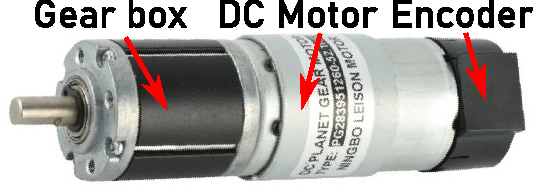
\includegraphics[scale=1]{src/img/fig1.pdf}
		\caption{Typical dc motor}
		\label{fig:Typical dc motor}
	\end{figure}
	
	\section{Modelling}
	
	\begin{figure}[ht]
		\centering
		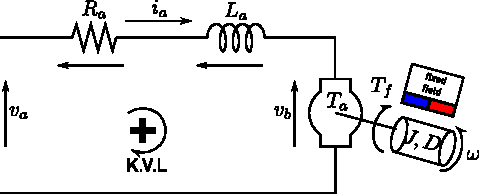
\includegraphics[scale=1.7]{src/img/fig2.pdf}
		\caption{dc motor model}
		\label{fig:dc motor model}
	\end{figure}
	
	\subsection{Electrical Part}
	\begin{equation}
		v_b(t) = K_b \dot{\theta}(t) = K_b \omega(t)
		\label{eq1}
	\end{equation}
	Where:
	\begin{itemize}
		\item {\makebox[1cm]{\(v_b(t)\)\hfill} is voltage at terminal conductor of motor }
		\item {\makebox[1cm]{\(K_b\)\hfill} is back emf constant}
		\item {\makebox[1cm]{\(\dot{\theta} = \omega\)\hfill} is angular velocity of motor}
	\end{itemize}
	
	\begin{equation}
		T_a = K_t i_a(t)
		\label{eq2}
	\end{equation}
	Where:
	\begin{itemize}
		\item {\makebox[1cm]{\(T_a\)\hfill} is rotor torque }
		\item {\makebox[1cm]{\(K_t\)\hfill} is motor torque}
		\item {\makebox[1cm]{\(i_a\)\hfill} is the current draw by motor}
	\end{itemize}
	\hfill\\
	By applying Kirchoff Voltage Law to the circuit loop in \autoref{fig:dc motor model}
	\begin{itemize}
		\item {\makebox[3.5cm]{\(v_a(t)\)\hfill} is input voltage from power source}
		\item {\makebox[3.5cm]{\(v_{resistance} = R_a i_a(t)\)\hfill} is voltage across resistance}
		\item {\makebox[3.5cm]{\(v_{inductor} = L_a \frac{di_a(t)}{dt}\)\hfill} is voltage across inductor}
	\end{itemize}
	
	\[v_a(t) - v_b(t) - R_a i_a(t) - L_a \frac{di_a(t)}{dt} = 0\]
	
	\begin{equation}
		\Rightarrow v_a(t) = v_b(t) + R_a i_a(t) + L_a \frac{di_a(t)}{dt}
		\label{eq3}
	\end{equation}
	Substitute \autoref{eq1} into \autoref{eq3}, we get:
	
	\begin{equation}
		v_a(t) = K_b \omega(t) + R_a i_a(t) + L_a \frac{di_a(t)}{dt}
		\label{eq4}
	\end{equation}
	In practical dc motor the \(L_a\) is very small (\(L_a \approx 0\)) and neglectable.
	
	\[v_a(t) = K_b \omega(t) + R_a i_a(t)\]
	
	\begin{equation}
		\Rightarrow \boxed{i_a(t) = \frac{v_a(t) - K_b \omega(t)}{R_a}}
		\label{eq5}
	\end{equation}
	
	\subsection{Mechanical Part}
	
	\begin{equation}
		T_a = T_f + J \dot{\omega}(t)
		\label{eq6}
	\end{equation}
	Where:
	\begin{itemize}
		\item {\makebox[1cm]{\(T_f\)\hfill} is torque of coulomb friction and viscous friction }
		\item {\makebox[1cm]{\(J\)\hfill} is moment of inertia}
	\end{itemize}
	We know that:
	\begin{equation}
		T_f = T_c sign[\omega(t)]+D\omega(t)
		\label{eq7}
	\end{equation}
	Where:
	\begin{itemize}
		\item {\makebox[1cm]{\(T_c\)\hfill} is coulomb friction torque}
		\item {\makebox[1cm]{\(D\)\hfill} is coefficient viscous friction}
	\end{itemize}
	Substitute \autoref{eq7} to \autoref{eq6}, we get:
	\[T_a = T_c sign[\omega(t)]+D\omega(t) + J \dot{\omega}(t)\]
	
	\subsubsection{Approximation of coulomb friction to zero \(T_c \approx 0\)}
	\begin{equation}
		T_a = D\omega(t) + J \dot{\omega}(t)
		\label{eq8}
	\end{equation}
	From \autoref{eq2}: \(T_a = K_t i_a(t)\) substitute to \autoref{eq8}:
	\[K_t i_a(t) = D\omega(t) + J \dot{\omega}(t)\]
	\begin{equation}
		\Rightarrow \boxed{i_a(t) = \frac{D\omega(t) + J \dot{\omega}(t)}{K_t}}
		\label{eq9}
	\end{equation}
	
	\subsubsection{Keep coulomb friction \(T_c\)}
	\begin{equation}
		\Rightarrow \boxed{i_a(t) = \frac{T_c sign[\omega(t)] + D\omega(t) + J \dot{\omega}(t)}{K_t}}
		\label{eq10}
	\end{equation}
	
	\section{Electrical and Mechanical combine}
	\subsection{Approximation of coulomb friction to zero \(T_c \approx 0\)}
	
	From \autoref{eq5} and \autoref{eq9}: Put it side by side:
	
	\[i_a(t) = i_a(t)\]
	\[\frac{v_a(t) - K_b \omega(t)}{R_a} = \frac{D\omega(t) + J \dot{\omega}(t)}{K_t}\]
	Get \(\dot{\omega}(t)\):
	
	\[\dot{\omega}(t) = \frac{\frac{(v_a(t) - K_b \omega(t))K_t}{R_a} - D\omega(t)}{J}\]
	\[\dot{\omega}(t) = \frac{(v_a(t) - K_b \omega(t))K_t}{R_a J} - \frac{D\omega(t)}{J}\]
	\[\dot{\omega}(t) = \frac{v_a(t) K_t - K_b K_t\omega(t)}{R_a J} - \frac{D\omega(t)}{J}\]
	Separate \(\omega(t)\) and \(v_a(t)\):
	
	\begin{equation}
		\boxed{\dot{\omega}(t) = - (\frac{K_b K_t + D R_a}{R_a J})\omega(t) + \frac{K_t}{R_a J}v_a(t)}
		\label{eq11}
	\end{equation}
	Let:
	\begin{itemize}
		\item {\makebox[4cm]{\(a = (\frac{K_b K_t + D R_a}{R_a J}) \omega(t)\)\hfill} \([1/s]\) }
		\item {\makebox[4cm]{\(b = \frac{K_t}{R_a J}\)\hfill} \([rad/s^2/V]\) }
	\end{itemize}
	We get lamped Parameter in a simplified form as:
	\begin{equation}
		\Rightarrow \boxed{\dot{\omega}(t) = - a\omega(t) + bv_a(t)}
		\label{eq12}
	\end{equation}
	
	
	\subsection{Keep coulomb friction \(T_c\)}
	\begin{equation}
		\boxed{\dot{\omega}(t) = - (\frac{K_b K_t + D R_a}{R_a J})\omega(t) + \frac{K_t}{R_a J}v_a(t) - \frac{T_c}{J}sign(\omega(t))}
		\label{eq13}
	\end{equation}
	Let:
	\begin{itemize}
		\item {\makebox[4cm]{\(a = (\frac{K_b K_t + D R_a}{R_a J})\)\hfill} \([1/s]\) }
		\item {\makebox[4cm]{\(b = \frac{K_t}{R_a J}\)\hfill} \([rad/s^2/V]\) }
		\item {\makebox[4cm]{\(c = \frac{T_c}{J}\)\hfill} \([.]\) }
	\end{itemize}
	We get lamped Parameter in a simplified form as:
	\begin{equation}
		\Rightarrow \boxed{\dot{\omega}(t) = - a\omega(t) + bv_a(t) - csign(\omega(t))}
		\label{eq14}
	\end{equation}
	
	\section{Simulation}
	
	In general, the equation \(\dot{\omega}(t) = - a\omega(t) + bv_a(t) - csign(\omega(t)\) is used to represent all the dc motor in the market. By modifying the parameters \(a, b, c\) will result in different dc motor.\\
	
	From equation \(\dot{\omega}(t) = - a\omega(t) + bv_a(t) - csign(\omega(t)\)
	\begin{itemize}
		\item {\makebox[1cm]{\(\dot{\omega}(t)\)\hfill} is the angular acceleration of dc motor and is the output of the system}
		\item {\makebox[1cm]{\(\omega(t)\) \hfill} is the angular velocity of dc motor and is the output of the system}
		\item {\makebox[1cm]{\(v_a(t)\)\hfill} is the input voltage to dc motor and is the input of the system}
	\end{itemize}
	
	\begin{figure}[ht]
		\centering
		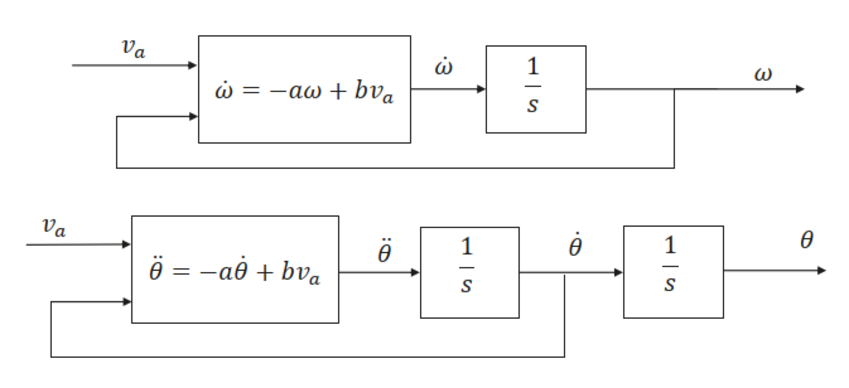
\includegraphics[scale=1]{src/img/fig3.pdf}
		\caption{Simulation Flow}
		\label{fig:Simulation Flow}
	\end{figure}
	\break
	\subsection{SIMULINK}
	
	\begin{figure}[ht]
		\centering
		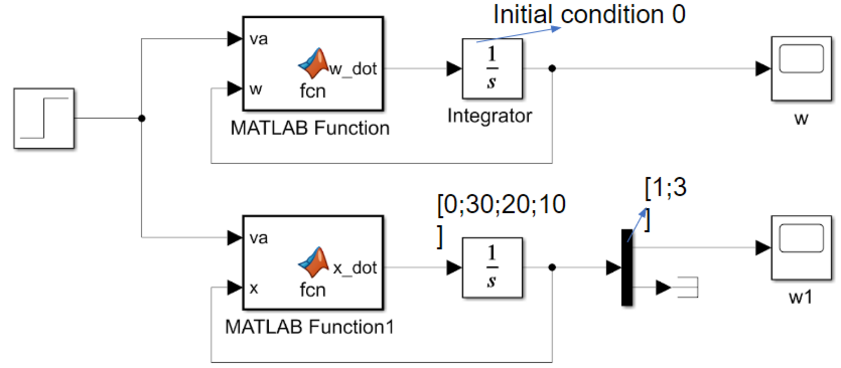
\includegraphics[scale=1]{src/img/fig4.pdf}
		\caption{SIMULINK Simulation Flow}
		\label{fig:SIMULINK Simulation Flow}
	\end{figure}

	\section{DC Motor 2nd Order Model ($ L_a $ is not Neglected)}
	\subsection{No Friction}
	From \autoref{eq4} and \autoref{eq9}, we have:
	\[\begin{split}
		v_a(t) &= K_b \omega(t) + R_a i_a(t) + L_a \frac{di_a(t)}{dt} \\
		i_a(t) &= \frac{D\omega(t) + J \dot{\omega}(t)}{K_t}
	\end{split}\]
	\[\begin{split}
		\frac{di_a(t)}{d(t)} &= \frac{d}{dt}\left(\frac{D\omega(t) + J \dot{\omega}(t)}{K_t}\right) \\
		&= \frac{1}{K_t}\frac{d}{dt}(D\omega(t) + J \dot{\omega}(t))\\
		&= \frac{1}{K_t} \frac{d}{dt}(D\omega(t)) + \frac{d}{dt}(J \dot{\omega}(t)) \\
		&= \frac{1}{K_t} (D\dot{\omega}(t) + J \ddot{\omega}(t))
	\end{split}\]
	We get:
	\begin{equation}
		v_a(t) = K_b \omega(t) + R_a \frac{D\omega(t) + J \dot{\omega}(t)}{K_t} + L_a\frac{1}{K_t} (D\dot{\omega}(t) + J \ddot{\omega}(t))
		\label{eq15}
	\end{equation}
	\[\begin{split}
		K_tv_a(t) &= K_tK_b \omega(t) + R_a (D\omega(t) + J \dot{\omega}(t)) + L_a (D\dot{\omega}(t) + J \ddot{\omega}(t)) \\
		K_tv_a(t) &= K_tK_b \omega(t) + R_a D\omega(t) + R_a J \dot{\omega}(t) + L_a D\dot{\omega}(t) + L_aJ \ddot{\omega}(t) \\
		K_tv_a(t) &= (K_tK_b + R_a D) \omega(t) + (R_a J + L_a D) \dot{\omega}(t) + L_aJ \ddot{\omega}(t) \\
		L_aJ \ddot{\omega}(t) &= -(K_tK_b + R_a D) \omega(t) - (R_a J + L_a D) \dot{\omega}(t) + K_tv_a(t) \\
		\ddot{\omega}(t) &= - \frac{R_a J + L_a D}{L_aJ} \dot{\omega}(t) -\frac{K_tK_b + R_a D}{L_aJ} \omega(t)  + \frac{K_t}{L_aJ}v_a(t) \\
	\end{split}\]
	Let:
	\begin{itemize}
		\item {\makebox[4cm]{\(a = \frac{R_a J + L_a D}{L_aJ}\)\hfill} \([.]\) }
		\item {\makebox[4cm]{\(b = \frac{K_tK_b + R_a D}{L_aJ}\)\hfill} \([.]\) }
		\item {\makebox[4cm]{\(c = \frac{K_t}{L_aJ}\)\hfill} \([.]\) }
	\end{itemize}
	We get lamped Parameter in a simplified form as:
	\begin{equation}
		\Rightarrow \boxed{\ddot{\omega}(t) = - a\dot{\omega}(t) - b\omega(t) + cv_a(t)}
		\label{eq16}
	\end{equation}

	\subsection{With Friction}
	From \autoref{eq4} and \autoref{eq10}, we have:
	\[\begin{split}
		v_a(t) &= K_b \omega(t) + R_a i_a(t) + L_a \frac{di_a(t)}{dt} \\
		i_a(t) &= \frac{T_c sign[\omega(t)] +D\omega(t) + J \dot{\omega}(t)}{K_t}
	\end{split}\]
	\[\begin{split}
		\frac{di_a(t)}{d(t)} &= \frac{d}{dt}\left(\frac{T_c sign[\omega(t)] +D\omega(t) + J \dot{\omega}(t)}{K_t}\right) \\
		&= \frac{1}{K_t} (D\dot{\omega}(t) + J \ddot{\omega}(t)) \leftarrow \text{derivative of sign function is 0}
	\end{split}\]
	We get:
	\begin{equation}
		v_a(t) = K_b \omega(t) + R_a \frac{T_c sign[\omega(t)] + D\omega(t) + J \dot{\omega}(t)}{K_t} + L_a\frac{1}{K_t} (D\dot{\omega}(t) + J \ddot{\omega}(t))
		\label{eq17}
	\end{equation}
	\[\begin{split}
		K_tv_a(t) &= K_tK_b \omega(t) + R_aT_c sign[\omega(t)] + R_aD\omega(t) + R_aJ \dot{\omega}(t)) + L_a D\dot{\omega}(t) + L_a J \ddot{\omega}(t) \\
		\ddot{\omega}(t) &= - \frac{R_a J + L_a D}{L_aJ} \dot{\omega}(t) -\frac{K_tK_b + R_a D}{L_aJ} \omega(t)  + \frac{K_t}{L_aJ}v_a(t) - \frac{R_aT_c}{L_aJ} sign[\omega(t)]\\
	\end{split}\]
	Let:
	\begin{itemize}
		\item {\makebox[4cm]{\(a = \frac{R_a J + L_a D}{L_aJ}\)\hfill} \([.]\) }
		\item {\makebox[4cm]{\(b = \frac{K_tK_b + R_a D}{L_aJ}\)\hfill} \([.]\) }
		\item {\makebox[4cm]{\(c = \frac{K_t}{L_aJ}\)\hfill} \([.]\) }
		\item {\makebox[4cm]{\(d = \frac{R_aT_c}{L_aJ}\)\hfill} \([.]\) }
	\end{itemize}
	We get lamped Parameter in a simplified form as:
	\begin{equation}
		\Rightarrow \boxed{\ddot{\omega}(t) = - a\dot{\omega}(t) - b\omega(t) + cv_a(t) - dsign(\omega(t))}
		\label{eq18}
	\end{equation}
\end{document}